\chapter{Layered network models}
\label{Layered-network-models}
In this chapter, we present the definition of the \texttt{LayeredNetwork} class, which encodes the support in \textsc{Line} for layered queueing networks. These models are extended queueing networks where servers, in order to process jobs, can issue synchronous and asynchronous calls among each other. The topology of call dependencies makes it possible to partition the model into a set of layers, each consisting of a subset of the resources. %We point to \cite{fran.ea09} and to the LQNS user manual for an introduction~\cite{lqns12}.

\section{LayeredNetwork object definition}
\label{layerednetwork-object-definition}
\subsection{Creating a layered network topology}
A layered queueing network consists of four types of elements: processors, tasks, entries and activities. An entry is a class of service specified through a finite sequence of activities, and hosted by a task running on a (physical) processor. A task is typically a software queue that models access to the capacity of the underpinning processor. Activities model either service demands required at the underpinning processor, or calls to entries exposed by some remote tasks.

To create our first layered network, we instantiate a new model as
\begin{lstlisting}
model = LayeredNetwork('myLayeredModel');
\end{lstlisting}
We now proceed to instantiate the static topology of processors, tasks and entries:
\begin{lstlisting}
P1 = Processor(model, 'P1', 1, SchedStrategy.PS);
P2 = Processor(model, 'P2', 1, SchedStrategy.PS);
T1 = Task(model, 'T1', 5, SchedStrategy.REF).on(P1);
T2 = Task(model, 'T2', 1, SchedStrategy.INF).on(P2);
E1 = Entry(model, 'E1').on(T1);
E2 = Entry(model, 'E2').on(T2);
\end{lstlisting}
Here, the \texttt{on} method specifies the associations between the elements, e.g., task \texttt{T1} runs on processor \texttt{P1}, and accepts calls to entry \texttt{E1}. Furthermore, the multiplicity of \texttt{T1} is 5, meaning that up to 5 calls can be simultaneously served by this element (i.e., 5 is the number of servers in the underpinning queueing system for \texttt{T1}). Note that both processors and tasks can be associated to the standard \textsc{Line} scheduling strategies, with the exception that \texttt{SchedStrategy.REF} should be used to denote the reference task, which has a similar meaning to the reference node in the \texttt{Network} object.

\subsection{Describing service times of entries}
The service demands placed by an entry on the underpinning processor is described in terms of execution of one or more activities. Although in tools such as LQNS activities can be associated to either entries or tasks, \textsc{Line} supports only the more general of the two options, i.e., the definition of activities of the level of tasks. In this case:
\begin{itemize}
\item Every task defines a collection of activities.
\item Every entry needs to specify an initial activity where the execution of the entry starts (the activity is said to be ``bound to the entry'') and a final activity, which upon completion terminates the execution of the entry.
\end{itemize}
For example, we can associate an activity to each entry as follows:
\begin{lstlisting}
A1 = Activity(model, 'A1', Exp(1.0)).on(T1).boundTo(E1).synchCall(E2,3.5);
A2 = Activity(model, 'A2', Exp(2.0)).on(T2).boundTo(E2).repliesTo(E2);
\end{lstlisting}
Here, \texttt{A1} is a task activity for \texttt{T1}, acts as initial activity for \texttt{E1}, consumes an exponential distributed time on the processor underpinning \texttt{T1}, and requires on average 3.5 synchronous calls to \texttt{E2} to complete. Each call to entry \texttt{E2} is served by the activity  \texttt{A2}, with a service time on the processor underneath \texttt{T2} given by an exponential distribution with rate $\lambda=2.0$.

At present, \textsc{Line} 2.0.0-ALPHA supports only synchronous calls. Support for asynchronous calls is available in older versions, e.g. \textsc{Line} 1.0.0. Extension of \textsc{Line} 2.0.0-ALPHA to asynchronous calls

\subsubsection{Activity graphs}
Often, it is useful to structure the sequence of activities carried out by an entry in a graph. Currently, \textsc{Line} supports this feature only for activities places in series. For example, we may replace the specification of the activities underpinning a call to \texttt{E2} as
\begin{lstlisting}
A20 = Activity(model, 'A20', Exp(1.0)).on(T2).boundTo(E2);
A21 = Activity(model, 'A21', Erlang.fitMeanAndOrder(1.0,2)).on(T2);
A22 = Activity(model, 'A22', Exp(1.0)).on(T2).repliesTo(E2);
T2.addPrecedence(ActivityPrecedence.Serial(A20, A21, A22));
\end{lstlisting}
such that a call to \texttt{E2} serially executes \texttt{A20}, \texttt{A21}, and \texttt{A22} prior to replying. Here, \texttt{A21} is chosen to be an Erlang distribution with given mean (1.0) and number of phases (2).

%Since activities are defined at task level, two entries can possibly share some of the task activities, making task-level activities more general than entry-level activities.

\subsection{Debugging and visualization}
The structure of a \texttt{LayeredNetwork} object can be graphically visualized as follows
\begin{lstlisting}
plot(model)
\end{lstlisting}
An example of the result is shown in the next figure. The figure shows two processors (\texttt{P1} and \texttt{P2}), two tasks (\texttt{T1} and \texttt{T2}), and three entries (\texttt{E1}, \texttt{E2}, and \texttt{E3}) with their associated activities. Both dependencies and calls are both shown as directed arcs, with the edge weight on call arcs corresponding to the average number of calls to the target entry. For example, \texttt{A1} calls \texttt{E3} on average 2.0 times.
\begin{figure}
  \centering
  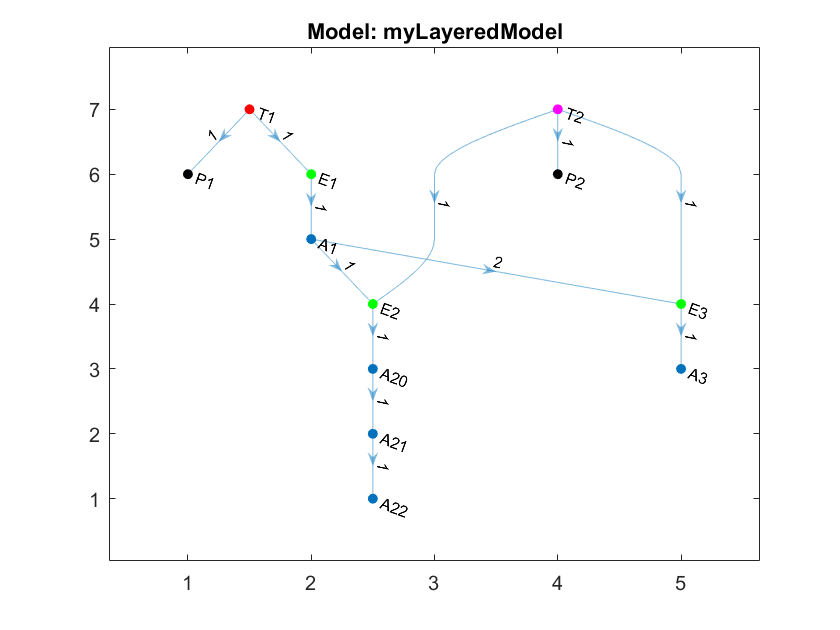
\includegraphics[width=8cm]{./images/lqnView.png}
  \caption{\texttt{LayeredNetwork.plot} method}\label{FIG_lqnView}
\end{figure}
As in the case of the \texttt{Network} class, the \texttt{getGraph} method can be called to inspect the structure of the \texttt{LayeredNetwork} object.

Lastly, the \texttt{jsimgView} and \texttt{jsimwView} methods can be used to visualize in JMT each layer. This can be done by first calling the \texttt{getLayers} method to obtain a cell array consisting of the \texttt{Network} objects, each one corresponding to a layer, and then invoking the \texttt{jsimgView} and \texttt{jsimwView} methods on the desired layer. This is discussed in more details in the next section.

\section{Decomposition into layers}
Layers are a form of decomposition where the influence of resources not explicitly represented in that layer is taken into account through an artificial delay station, placed in a closed loop to the resources~\cite{roli.sevc95}. This artificial delay is used to model the inter-arrival time between calls from resources that belong to other layers.

\subsection{Running a decomposition}
The current version of \textsc{Line} adopts SRVN-type layering~\cite{lqns12}, whereby a layer corresponds to one and only one resource, either a processor or a task. The only exception are reference tasks, which can only appear as clients to their processors.
The \texttt{getLayers} method returns a cell array consisting of the \texttt{Network} objects corresponding to each layer
\begin{lstlisting}
layers = model.getLayers()
\end{lstlisting}
Within each layer, classes are used to model the time a job spends in a given activity or call, with synchronous calls being modeled by classed with label including an arrow, e.g., \texttt{'AS1=>E3'} is a closed class used represent synchronous calls from activity \texttt{AS1} to entry \texttt{E3}. Artificial delays and reference nodes are modelled as a delay station named \texttt{'Clients'}, whereas the task or processor assigned to the layer is modelled as the other node in the layer.

\subsection{Initialization and update}
\label{initialization-and-update}
In general, the parameters of a layer will depend on the steady-state solution of an other layer, causing a cyclic dependence that can be broken only after the model is analyzed by a solver. In order to assign parameters within each layer prior to its solution, the \texttt{LayeredNetwork} class uses the \texttt{initDefault} method, which sets the value of the artificial delay to simple operational analysis bounds~\cite{LazZGS84}.

The layer parameterization depends on a subset of performance indexes stored in a \texttt{param} structure array within the \texttt{LayeredNetwork} class. After initialization, it is possible to update the layer parameterization for example as follows
\begin{lstlisting}
layers = model.getLayers();
for l=1:model.getNumberOfLayers()
    AvgTableByLayer{l} = SolverMVA(layers{l}).getAvgTable;
end
model.updateParam(AvgTableByLayer);
model.refreshLayers;
\end{lstlisting}
Here, the \texttt{refreshParam} method updates the \texttt{param} structure array from a cell array of steady-state solutions for the \texttt{Network} objects in each layer. Subsequently, the \texttt{refreshLayers} method enacts the new parameterization across the \texttt{Network} objects in each layer.

\section{Solvers}
\textsc{Line} offers two solvers for the solution of a \texttt{LayeredNetwork} model consisting in its own native solver (\texttt{LN}) and a wrapper (\texttt{LQNS}) to the LQNS solver~\cite{lqns12}. The latter requires a distribution of LQNS to be available on the operating system command line.

The solution methods available for \texttt{LayeredNetwork} models are similar to those for \texttt{Network} objects. For example, the \texttt{getAvgTable} can be used to obtain a full set of mean performance indexes for the model, e.g.,
\begin{lstlisting}
>> AvgTable = SolverLQNS(model).getAvgTable
AvgTable =
  8x6 table
    Node     NodeType       QLen        Util      RespT      Tput
    ____    ___________    _______    ________    _____    ________
    'P1'    'Processor'        NaN    0.071429     NaN          NaN
    'T1'    'Task'         0.28571    0.071429     NaN     0.071429
    'E1'    'Entry'        0.28571    0.071429       4     0.071429
    'A1'    'Activity'     0.28571    0.071429       4     0.071429
    'P2'    'Processor'        NaN     0.21429     NaN          NaN
    'T2'    'Task'         0.21429     0.21429     NaN      0.21429
    'E2'    'Entry'        0.21429     0.21429       1      0.21429
    'A2'    'Activity'     0.21429     0.21429       1      0.21429
\end{lstlisting}
Note that in the above table, some performance indexes are marked as \texttt{NaN} because they are not defined in a layered queueing network. Further, compared to the \texttt{getAvgTable} method in \texttt{Network} objects, \texttt{LayeredNetwork} do not have an explicit differentiation between stations and classes, since in a layer a task may either act as a server station or a client class.

The main challenge in solving layered queueing networks through analytical methods is that the parameterization of the artificial delays depends on the steady-state performance of the other layers, thus causing a cyclic dependence between input parameters and solutions across the layers. Depending on the solver in use, such issue can be addressed in a different way, but in general a decomposition into layers will remain parametric on a set of response times, throughputs and utilizations.

This issue can be resolved through solvers that, starting from an initial guess, cyclically analyze the layers and update their artificial delays on the basis of the results of these analyses. Both \texttt{LN} and \texttt{LQNS} implement this solution method. Normally, after a number of iterations the model converges to a steady-state solution, where the parameterization of the artificial delays does not change after additional iterations.

\subsection{\texttt{LQNS}}
The LQNS wrapper operates by first transforming the specification into a valid LQNS XML file. Subsequently, LQNS calls the solver and parses the results from disks in order to present them to the user in the appropriate \textsc{Line} tables or vectors. The \texttt{options.method} can be used to configure the LQNS execution as follows:
\begin{itemize}
\item \texttt{options.method='std'} or \texttt{'lqns'}: LQNS analytical solver with default settings.
\item \texttt{options.method='exact'}: the solver will execute the standard LQNS analytical solver with the exact MVA method.
\item \texttt{options.method='srvn'}: LQNS analytical solver with SRVN layering.
\item \texttt{options.method='srvnexact'}: the solver will execute the standard LQNS analytical solver with SRVN layering and  the exact MVA method.
\item \texttt{options.method='lqsim'}: LQSIM simulator, with simulation length specified via the \texttt{samples} field (i.e., with parameter \texttt{-A options.samples, 0.95}).
\end{itemize}

Upon invocation, the \texttt{lqns} or \texttt{lqsim} commands will be searched for in the system path. If they are unavailable, the termination of \texttt{SolverLQNS} will interrupt.

\subsection{\texttt{LN}}
The native \texttt{LN} solver iteratively applies the layer updates until convergence of the steady-state measures. Since updates are parametric on the solution of each layer, \texttt{LN} can apply any of the \texttt{Network} solvers described in the solvers chapter to the analysis of individual layers, as illustrated in the following example for the \texttt{MVA} solver
\begin{lstlisting}
options = SolverLN.defaultOptions;
mvaopt = SolverMVA.defaultOptions;
SolverLN(model, @(layer) SolverMVA(layer, mvaopt), options).getAvgTable
\end{lstlisting}
Options parameters may also be omitted. The \texttt{LN} method converges when the maximum relative change of mean response times across layers from the last iteration is less than \texttt{options.iter\_tol}.

\section{Model import and export}
A \texttt{LayeredNetwork} can be easily read from, or written to, a XML file based on the LQNS meta-model format\footnote{\url{https://raw.githubusercontent.com/layeredqueuing/V5/master/xml/lqn.xsd}}. The read operation can be done using a static method of the \texttt{LayeredNetwork} class, i.e.,
\begin{lstlisting}
model = LayeredNetwork.parseXML(filename)
\end{lstlisting}
Conversely, the write operation is invoked directly on the model object
\begin{lstlisting}
model.writeXML(filename)
\end{lstlisting}
In both examples, \texttt{filename} is a string including both file name and its path.

Finally, we point out that it is possible to export a LQN in the legacy SRVN file format\footnote{\url{http://www.sce.carleton.ca/rads/lqns/lqn-documentation/format.pdf}} by means of the \texttt{writeSRVN(filename)} function.

%\section{Feature comparison}
%
%\begin{table}[thbp]
%\begin{center}
%\begin{tabular}{|c|c|c|}
%\hline
%Feature & LQNS & LN \\
%\hline
%FULL-ACCESS & yes & ? \\
%Device scheduling & FHPS & FRS,... \\
%Task scheduling & FH & FRS,... \\
%Open arrivals & yes & no \\
%MULTI & yes & yes \\
%Infinite servers & yes & yes \\
%SERV-PATTERN & SD & ? \\
%VAR & yes & ? \\
%PAR & yes & no \\
%REPL & yes & ? \\
%ASYNC & yes & no \\
%Forwarding & yes & no \\
%FAST, INTERLOCK & yes & no \\
%\hline
%\end{tabular}
%\end{center}
%\label{TAB_lqn_solver_features}
%\caption{Layered solver features}
%\end{table}
